\documentclass{beamer}
\usepackage{amssymb}
\usepackage{graphicx}
\usepackage{wasysym}
\usetheme{Berlin}


\title[Emisi\'on de la fotosfera]{\textbf{Emisi\'on de la fotosfera}}
\author{Antonio Galv\'an}
\date{5 Mayo 2014}
\institute{Instituto de Astronom\'ia\\ Facultad
 de Ciencias\\ U.N.A.M.}

\begin{document}
\begin{frame}
\titlepage
\end{frame}

% % % % % % % % % % % % % % % % % % % % % % % % % % % % % % % % % % % % %
% % % % % % % % % % % % % Segunda diapositiva % % % % % % % % % % % % % %
% % % % % % % % % % % % % % % % % % % % % % % % % % % % % % % % % % % % % 

\begin{frame}
\frametitle{\'Indice}
\tableofcontents
\end{frame}

% % % % % % % % % % % % % % % % % % % % % % % % % % % % % % % % % % % % %
% % % % % % % % % % % % % Tercera diapositiva % % % % % % % % % % % % % %
% % % % % % % % % % % % % % % % % % % % % % % % % % % % % % % % % % % % %


\section{En general}

\begin{frame}
\frametitle{En general:} 
Se cree a lo largo de muchas observaciones que los GRB's surgen 
de la disipaci\'on de energ\'ia cin\'etica de un flujo relativista,
 original de un objeto central compacto.\\
Esta energ\'ia disipada es convertida en electrones energ\'eticos que
producen fotones altamente energ\'eticos por medio de radiaci\'on Sincrotron y 
Compton Inverso.
\end{frame}


% % % % % % % % % % % % % % % % % % % % % % % % % % % % % % % % % % % % %
% % % % % % % % % % % % % Cuarta diapositiva  % % % % % % % % % % % % % % 
% % % % % % % % % % % % % % % % % % % % % % % % % % % % % % % % % % % % %


\section{Y la fotosfera ?`qu\'e rol tiene?}
\begin{frame}
\frametitle{?`Y la fotosfera ¿qu\'e rol tiene?}
	\begin{columns}
	
		\begin{column}{5cm}
		En un modelo c\'omo lo es el termonuclear en el que propone que el material acretado
		de un sistema binario o de una estrella de neutrones peque\~na con un entorno altamente
		denso.
		\end{column}
		
		\begin{column}{5cm}
		En el modelo de la estrella de neutrones formada por una capa de hidr\'ogeno ($H$) en la capa
		m\'as externa, seguida de una capa de helio ($He$) y metales por debajo de \'esta con una densidad
		de $10^{7}g cm^{-2}$ y $T\backsim 10^{7}K $ los electrones se degeneran.\\
		De esta manera se genera una combusti\'on nuclear.
		\end{column}	
	\end{columns}
\end{frame}


% % % % % % % % % % % % % % % % % % % % % % % % % % % % % % % % % % % % %
% % % % % % % % % % % % % Quinta diapositiva  % % % % % % % % % % % % % %
% % % % % % % % % % % % % % % % % % % % % % % % % % % % % % % % % % % % %


\begin{frame}
	\begin{columns}
	
		\begin{column}{5cm}
			\begin{figure}
				\centering
				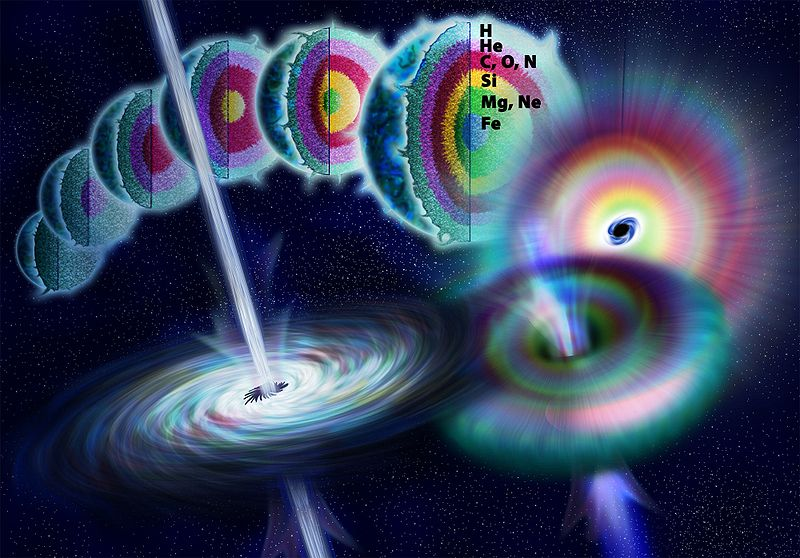
\includegraphics[scale=0.75]{neutronStar.jpg}
				\caption{Distintos procesos de la estrella de neutrones.}
			
			\end{figure}
		\end{column}
		
		\begin{column}{5cm}
		De tal forma de que el hidr\'ogeno se  por CNO no limitado y por medio de electrones 
		capturados por protones.\\ La tasa m\'inima de acreci\'on es de $\backsim 10^{15}M_{\astrosun}km^{-2}yr^{-1}$.\\
		Cu\'ando la temperatura alcanza $\backsim 10^{8}K $ la capa de $He$
		explota generando la cantidad necesaria para originar un GRB.
		\end{column}	
	\end{columns}
\end{frame}


% % % % % % % % % % % % % % % % % % % % % % % % % % % % % % % % % % % % %
% % % % % % % % % % % % % Sexta diapositiva % % % % % % % % % % % % % % %
% % % % % % % % % % % % % % % % % % % % % % % % % % % % % % % % % % % % %


\begin{frame}
	\begin{columns}
	
		\begin{column}{5cm}
		La capa de $He$ se quema de manera muy r\'apida, dentro de los $10^{-2}s$. La energ\'ia termonuclear
		se libera a la atm\'osfera y una vez ah\'i disipan su energ\'ia generando un campo el\'ectrico en \'optico.\\
		Dado que los electrones est\'an acelerados, por medio de Compton inverso producen un
		destello de rayo gamma (GRB), con fotones del cuerpo negro.\\
		Estos GRB de cientos de $KeV$ son intensos a trav\'es de las lineas del
		campo magn\'etico y escapan libremente por los polos.
		\end{column}	

		\begin{column}{5cm} 
			\begin{figure}
				\centering
				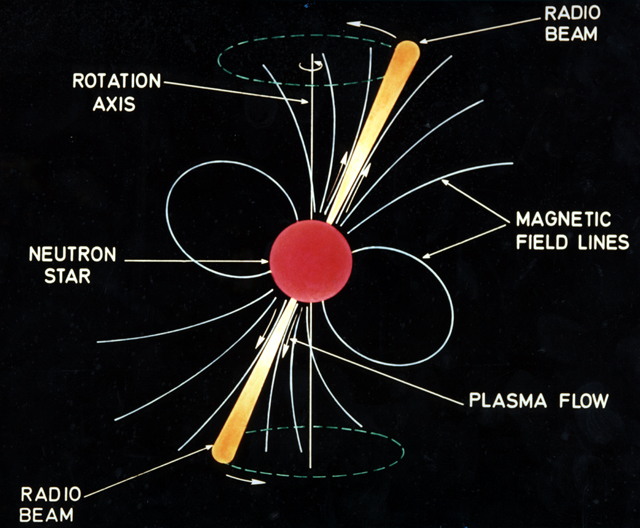
\includegraphics[scale=0.25]{expulsiondeljet.jpg}
				\caption{Observamos c\'omo toda esa energ\'ia corre libremente
				por las lineas del campo magn\'etico.}
			\end{figure}
		\end{column}	
	\end{columns}
\end{frame}


% % % % % % % % % % % % % % % % % % % % % % % % % % % % % % % % % % % % %
% % % % % % % % % % % % % Septima diapositiva % % % % % % % % % % % % % %
% % % % % % % % % % % % % % % % % % % % % % % % % % % % % % % % % % % % %



\begin{frame}
	\begin{columns}
	
		\begin{column}{5cm}
			\begin{figure}
				\centering
				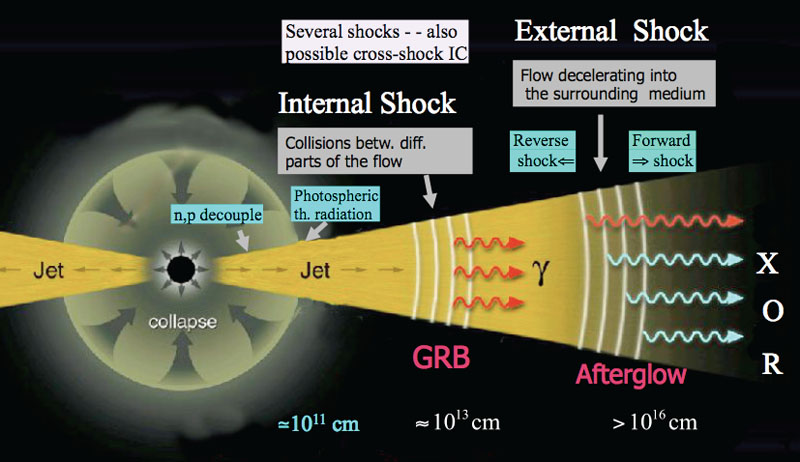
\includegraphics[scale=0.2]{figure1.jpg}
				\caption{Observemos las distancias a las que se
				genera cada momento.}
			\end{figure}
		\end{column}
		
		
		\begin{column}{5cm}
		Los fotones experimentan una dispersi\'on Compton en electrones fr\'ios y crean una subpoblaci\'on de electrones
		calientes que emiten en radiaci\'on de sincrotr\'on, que resulta ser t\'ermica y que corresponde a la energ\'ia t\'ipica
		de excitaci\'on de los electrones: $kT_{s} \backsim mc^{2}$
		\end{column}	
	\end{columns}
\end{frame}


% % % % % % % % % % % % % % % % % % % % % % % % % % % % % % % % % % % % %
% % % % % % % % % % % % % Octava  diapositiva % % % % % % % % % % % % % % 
% % % % % % % % % % % % % % % % % % % % % % % % % % % % % % % % % % % % %


\begin{frame}
	\begin{columns}
	
		\begin{column}{5cm}
		El espectro emitido por el sistema de iluminaci\'on de esta fotosfera
		es la suma de un cuerpo negro con la temperatura de algunos $KeV$ y la
		radiaci\'on de sincrotr\'on considerada c\'omo t\'ermica con temperatura
		$kT_{s} \backsim mc^{2}$. Esa energ\'ia liberada esta en el rango de 
		$10^{37} - 10^{49} erg.$ implicando distancias entre unos cientos de parsecs
		y $1-2 kpc$
		\end{column}
		
		
		\begin{column}{5cm}
		La tasa de acreci\'on siendo un flujo de rayos es de  $3 x 10^{-14}erg cm^{-2}s $.
		Para distancias de $1 kpc$ es demasiado baja para los limites deducidos por las
		observaciones de Einstein.
		
		\end{column}	
	\end{columns}
\end{frame}


% % % % % % % % % % % % % % % % % % % % % % % % % % % % % % % % % % % % %
% % % % % % % % % % % % % Novena  diapositiva % % % % % % % % % % % % % % 
% % % % % % % % % % % % % % % % % % % % % % % % % % % % % % % % % % % % %

\section{?`Entonces?}

\begin{frame}{?`Y en cristiano, espa\~nol, humano?}
Poniendo c\'omo referencia el modelo termonuclear y nuestra estrella de neutrones, pasa que
las capas de H y He generan combustión, cu\'ando la temperatura llega a los $10{8}K$ la capa
de He acaba de explotar, se genera un disco de acreci\'on y radia un cuerpo negro.

Pues la estrella esta colapsando por a ra\'iz de la combusti\'on y la gravedad que justo, por
donde est\'an las lineas del campo magn\'etico de la estrella se va a vencer as\'i logrando salir
toda esa energ\'ia que se venia acumulando.
	\begin{figure}
		\centering
		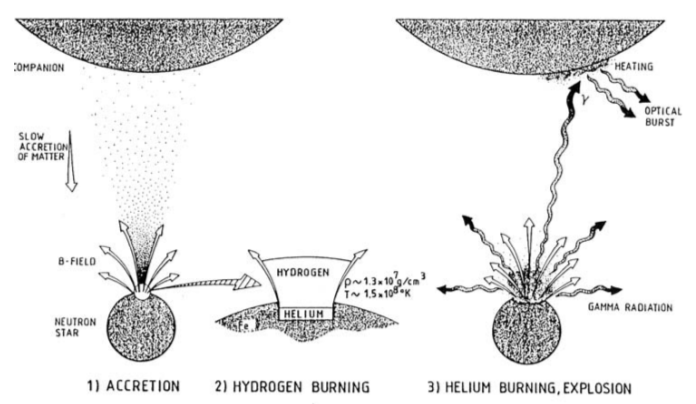
\includegraphics[scale=0.2]{creacionGRB.png}
		\caption{Ilustraci\'on del modelo termonuclear en un sistema binario.}
	\end{figure}
\end{frame}

% % % % % % % % % % % % % % % % % % % % % % % % % % % % % % % % % % % % % % % % % % % % % % % % % % %
% % % % % % % % % % % % % % %Decima diapositiva % % % % % % % % % % % % % % % % % % % % % % % % % % %
% % % % % % % % % % % % % % % % % % % % % % % % % % % % % % % % % % % % % % % % % % % % % % % % % % %


\begin{frame}
\frametitle{Aj\'a ?`Y luego que?}
	\begin{columns}
		\begin{column}{5cm}
		Resulta que a una distanc\'ia entre los ${10^{10 \backsim 12} cm}$ se forma la
		fotosfera de nuestro GRB.
		
		?`Que importa?
		
		Ah\'i pasan dos fen\'omenos interesantes, pues a partir de ah\'i, capaz (unas m\'as lentas
		que otras) van a salir, las m\'as r\'apidas alcanzaran a las lentas, dando lugar a los choques
		internos, esto va a suceder entre los ${10^{12 \backsim 15} cm}$ lo que pasa ah\'i 
		
		\end{column}
		
		\begin{column}{5cm}
		
			Resulta que cu\'ando dos "shell" o caparazones, como los de la figura chocan "calientan" la materia
			\begin{figure}
				\centering
				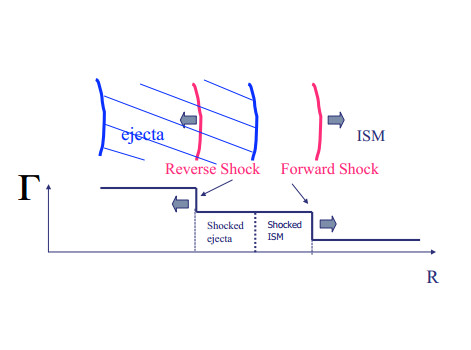
\includegraphics[scale=0.25]{choques.jpg}
				\caption{Ilustraci\'on de los choques internos.}
			\end{figure}
		\end{column}	
	\end{columns}
\end{frame}


% % % % % % % % % % % % % % % % % % % % % % % % % % % % % % % % % % % % % % % % % % % % % % % % % % %
% % % % % % % % % % % % % % % % % %Decima primer diapositiva% % % % % % % % % % % % % % % % % % % % %
% % % % % % % % % % % % % % % % % % % % % % % % % % % % % % % % % % % % % % % % % % % % % % % % % % %

\begin{frame}
	\begin{columns}
		\begin{column}{5cm}
		Ya que interaccionan esta capas, convierten toda esta energ\'ia cin\'etica
		en movimientos aleatorios de part\'iculas
		de tal forma que se va a liberar m\'as energ\'ia.
		
		Ya que estas part\'iculas se desplazan a 
		velocidades relativistas y conservan aun el campo magn\'etico (dado que desde un inicio hablamos de part\'iculas cargadas)
		Se genera la radiaci\'on de Sincr\'otron.
		
		Por medio de estas interacciones (de los choques internos) se genera un espectro 
		de luminiscencia.
		\end{column}
		
		\begin{column}{5cm}
			\begin{figure}
				\centering
				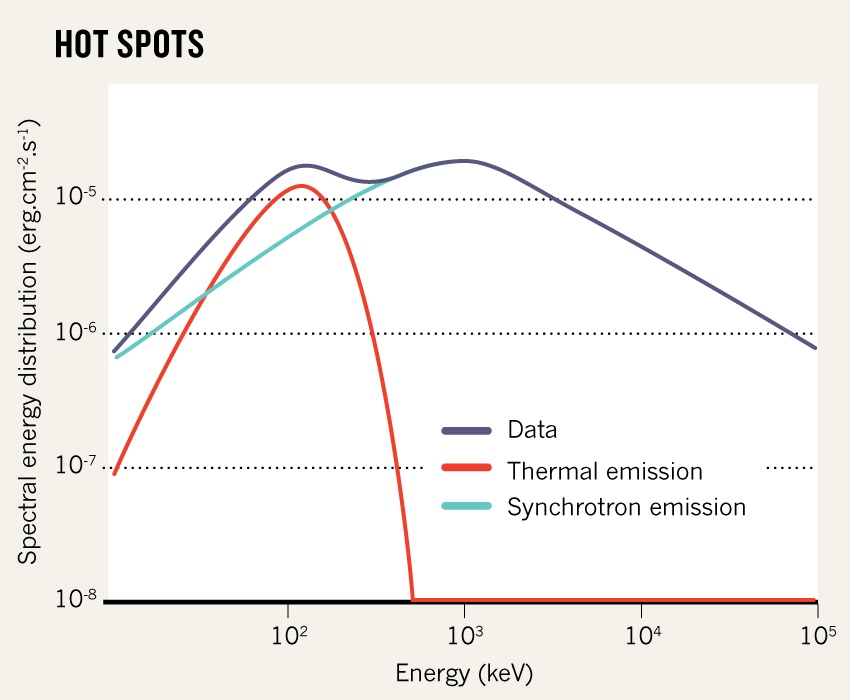
\includegraphics[scale=0.15]{grb-spectrum1.jpg}
				\caption{Actividad esperada de la emisi\'on de Sincrotr\'on.}
			\end{figure}
		\end{column}	
	\end{columns}
\end{frame}


% % % % % % % % % % % % % % % % % % % % % % % % % % % % % % % % % % % % % % % % % % % % % % % % % % %
% % % % % % % % % % % % % % % % % %Decima segunda diapositiva% % % % % % % % % % % % % % % % % % % % %
% % % % % % % % % % % % % % % % % % % % % % % % % % % % % % % % % % % % % % % % % % % % % % % % % % %


		

\begin{frame}
	\begin{columns}
		\begin{column}{5cm}
		Una vez que ha pasado todo ese proceso
				en una distancia mayores de $10^{15 \backsim 16 cm.}$ Suceden los choques externos, es decir, la interacci\'on del jet con el medio interestelar.
				
				Aqu\'i sucede el efecto de Compton inverso, lo que significa que esos fotones que ven\'ian con una baja energ\'ia la ganen por medio electrones. Así es, esos electrones que ven\'ian a velocidades relativistas de los choques internos le den energ\'ia a esos fotones y estos electrones la pierden.
		
		\end{column}
		
		\begin{column}{5cm}
			\begin{figure}
				\centering
				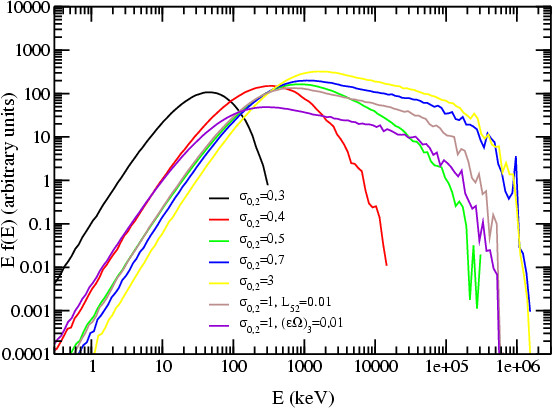
\includegraphics[scale=0.25]{img69.jpg}
				\caption{Comportamiento del Compton inverso.}
			\end{figure}
		\end{column}	
	\end{columns}
\end{frame}


% % % % % % % % % % % % % % % % % % % % % % % % % % % % % % % % % % % % % % % % % % % % % % % % % % %
% % % % % % % % % % % % % % % % % %Decima tercer diapositiva% % % % % % % % % % % % % % % % % % % % %
% % % % % % % % % % % % % % % % % % % % % % % % % % % % % % % % % % % % % % % % % % % % % % % % % % %



\begin{frame}
\section{Al final}
\frametitle{Al final}
	\begin{columns}
		\begin{column}{5cm}
		Podemos observar que a ra\'iz de lo que
		se genera en la fotosfera se describe un
		gran comportamiento de un GRB.\\
		
		Tengo que mencionar que tambi\'en hay 
		fotosferas con propiedades no t\'ermicas.\\
		
		Tambi\'en he omitido muchos procesos que
		se llevan a cabo dentro de la fotosfera y tambi\'en hay muchos procesos que se est\'an proponiendo sobre esta misma.
		\end{column}
		
		\begin{column}{5cm}
			\begin{figure}
				Gracias por su atenci\'on
			\end{figure}
		\end{column}	
	\end{columns}
\end{frame}

\end{document}
